\section{Real World Smart Traffic}

Die Umweltbelastungen durch Treibhausgase ist im vergangen Jahrhundert auf ein bedrohliches Maß für unseren Klima angewachsen. Die Auswirkungen werden in der Weltgesellschaft gerne mit dem Schlagwort der Erderwärmung beschrieben. Im Jahre 2002 hat die EU das Kyoto-Protokoll ratifiziert, Bis zum Jahr 2030 sollen sich die Treibhausgas -Emissionen um 40\% gegenüber dem Jahr 1990 verringern. 

\begin{itemize} 
\item Pariser Klimakonferenz 2015 / 195 Staaten globale Staatengemeinschaft  /gleiches Ziel
\item Ziel: Globale Erwärmung auf unter 2 Grad Celsius / vorindustrielles Niveau 
\item Leitbild für deutsche Klimaschutzpolitik der Bundesregierung
\item Treibhausgaseffekte in Deutschland
\end{itemize}

\begin{figure}[ht]
	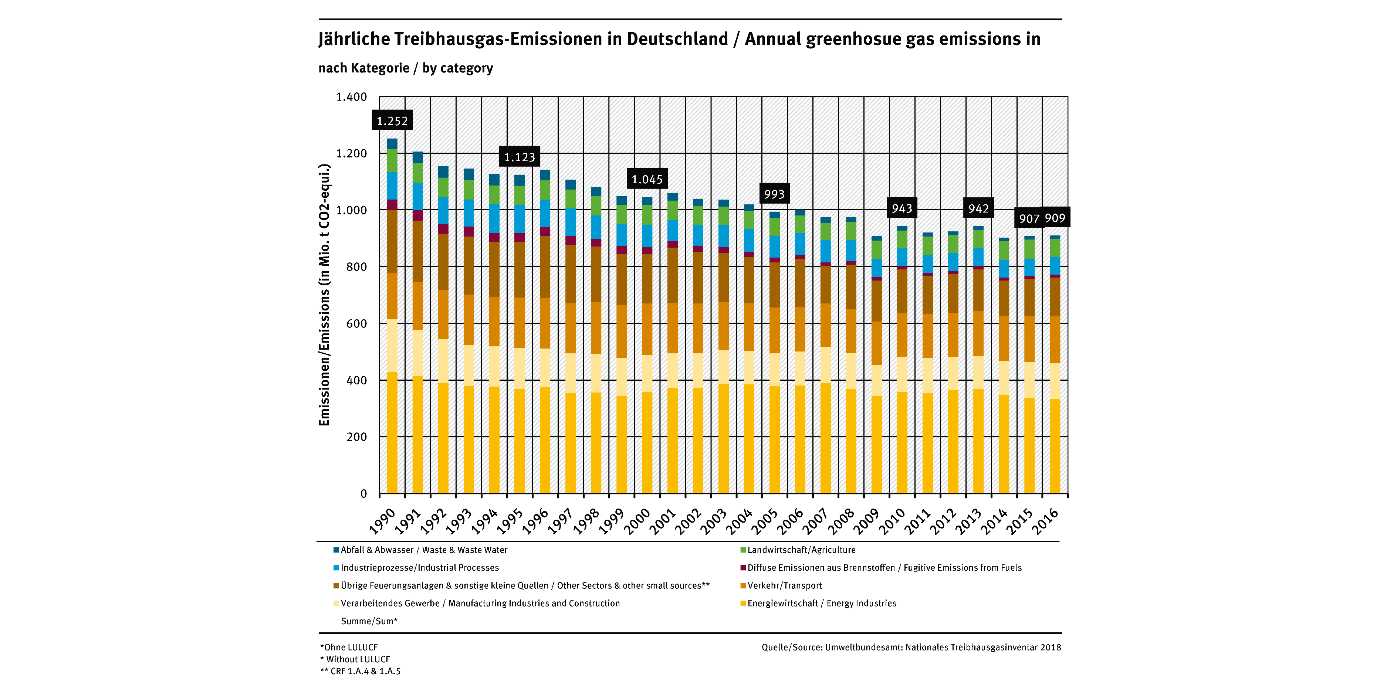
\includegraphics[width=\textwidth]{images/jaehrlicheTreibhausEmissionen.png}
	\caption{Entwicklung der jährlichen Treibhausemissionen in Deutschland}
	\label{fig2}
\end{figure}

-	allein der technische Fortschritte in Motorentechnik reicht nicht aus -> immer mehr Autos

Seit Jahren wird ein Anstieg des Verkaufsaufkommens auf deutschen Straßen verzeichnet. Unterstützt wird diese Feststellung durch die steigende Anzahl der in Deutschland angemeldeten Pkw. Laut dem Statistikinstitut „statista“ hat sich die Zahl gemeldeter Fahrzeuge seit 1960 von knapp 4,5 Millionen auf heute 46 Millionen erhöht [1]. Die Jahresbilanz 2018 des Kraftfahrtbundesamt weißt 63,7 Millionen zugelassene Fahrzeuge aus [2].  

-	speziell durch Transportmittel, welche mit Verbrennungsmotoren angetrieben ein Problem

[QUELLE: https://www.umweltbundesamt.de/themen/klima-energie/klimaschutz-energiepolitik-in-deutschland/treibhausgas-emissionen/emissionsquellen]

-	Einsparpotential im Verkehr mit über 40\% bewertet


\begin{figure}[ht]
	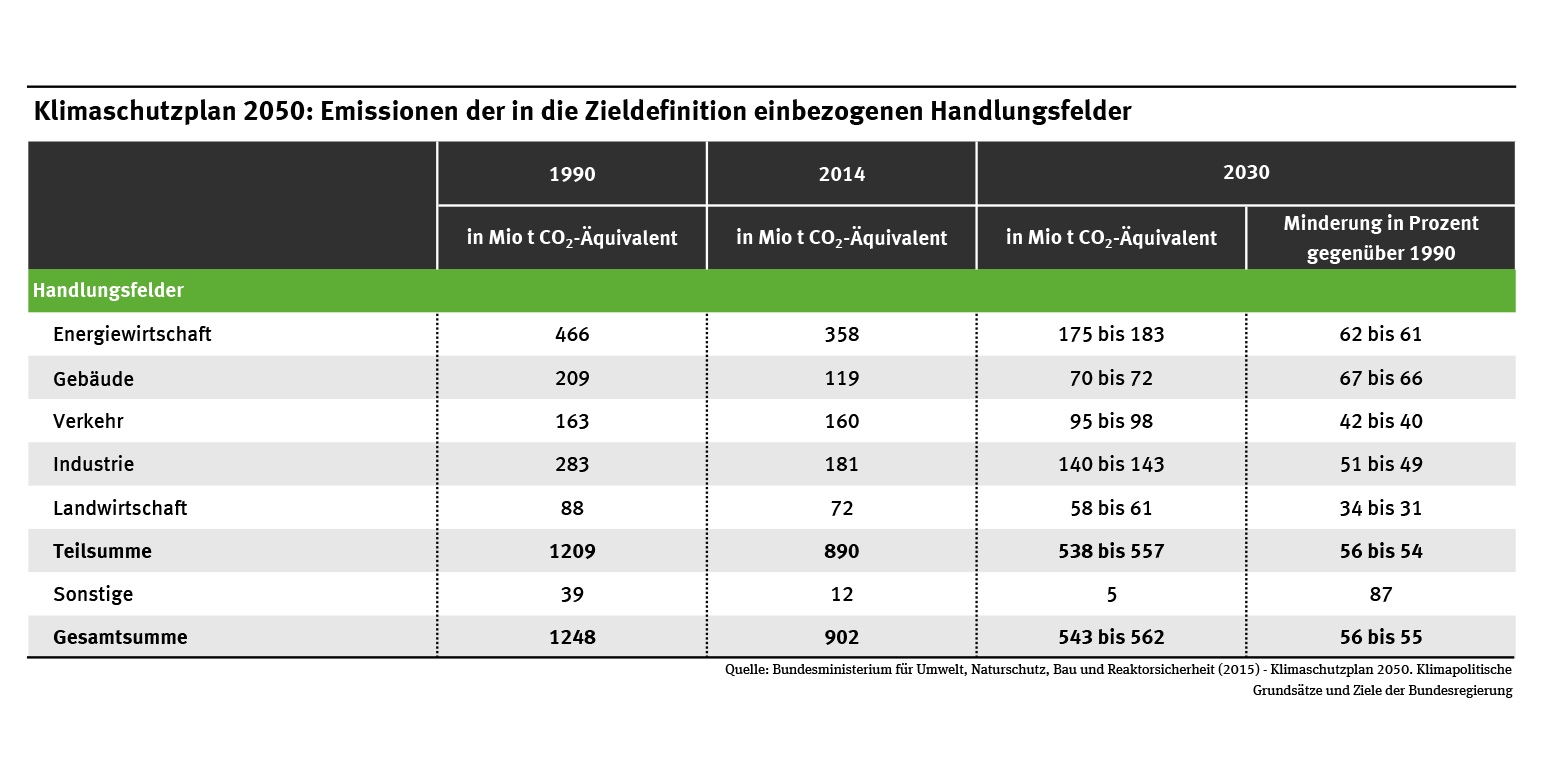
\includegraphics[width=\textwidth]{images/klimaschutzplan2050.png}
	\caption{Klimaschutzplan 2050}
	\label{fig2}
\end{figure}
[QUELLE: https://www.umweltbundesamt.de/daten/klima/klimaschutzziele-deutschlands]

4)	Santander in Spanien – Vorzeigestadt – 20 000 Sensoren

https://www.wiwo.de/adv/telekom-digitalisierung/insights/smart-city-wettrennen-um-die-stadt-der-zukunft/19313878.html



-	Probleme/Hindernisse
1)	Kostenpunkt
2)	Datenschutz/Rechtliches -> Missbrauch
3)	Angreifbar -> Sicherheitsrisiko



\clearpage
